
\documentclass{Configuration_Files/PoliMi3i_thesis}

%------------------------------------------------------------------------------
%	REQUIRED PACKAGES AND  CONFIGURATIONS
%------------------------------------------------------------------------------

% CONFIGURATIONS
\usepackage{parskip} % For paragraph layout
\usepackage{setspace} % For using single or double spacing
\usepackage{emptypage} % To insert empty pages
\usepackage{multicol} % To write in multiple columns (executive summary)
\setlength\columnsep{15pt} % Column separation in executive summary
\setlength\parindent{0pt} % Indentation
\raggedbottom  

% PACKAGES FOR TITLES
\usepackage{titlesec}
% \titlespacing{\section}{left spacing}{before spacing}{after spacing}
\titlespacing{\section}{0pt}{3.3ex}{2ex}
\titlespacing{\subsection}{0pt}{3.3ex}{1.65ex}
\titlespacing{\subsubsection}{0pt}{3.3ex}{1ex}
\usepackage{color}

% PACKAGES FOR LANGUAGE AND FONT

\usepackage[utf8]{inputenc} % UTF8 encoding
\usepackage[T1]{fontenc} % Font encoding
\usepackage[11pt]{moresize} % Big fonts

% PACKAGES FOR IMAGES
\usepackage{graphicx}
\usepackage{transparent} % Enables transparent images
\usepackage{eso-pic} % For the background picture on the title page
\usepackage{subfig} % Numbered and caption subfigures using \subfloat.
\usepackage{tikz} % A package for high-quality hand-made figures.
\usetikzlibrary{}
\graphicspath{{./Images/}} % Directory of the images
\usepackage{caption} % Coloured captions
\usepackage{xcolor} % Coloured captions
\usepackage{amsthm,thmtools,xcolor} % Coloured "Theorem"
\usepackage{float}

% STANDARD MATH PACKAGES
\usepackage{amsmath}
\usepackage{amsthm}
\usepackage{amssymb}
\usepackage{amsfonts}
\usepackage{bm}
\usepackage[overload]{empheq} % For braced-style systems of equations.
\usepackage{fix-cm} % To override original LaTeX restrictions on sizes

% PACKAGES FOR TABLES
\usepackage{tabularx}
\usepackage{longtable} % Tables that can span several pages
\usepackage{colortbl}

% PACKAGES FOR ALGORITHMS (PSEUDO-CODE)
\usepackage{algorithm}
\usepackage{algorithmic}

% PACKAGES FOR REFERENCES & BIBLIOGRAPHY
\usepackage[colorlinks=true,linkcolor=black,anchorcolor=black,citecolor=black,filecolor=black,menucolor=black,runcolor=black,urlcolor=black]{hyperref} % Adds clickable links at references
\usepackage{cleveref}
\usepackage[square, numbers, sort&compress]{natbib} % Square brackets, citing references with numbers, citations sorted by appearance in the text and compressed
\bibliographystyle{abbrvnat} % You may use a different style adapted to your field

% OTHER PACKAGES
\usepackage{pdfpages} % To include a pdf file
\usepackage{afterpage}
\usepackage{lipsum} % DUMMY PACKAGE
\usepackage{fancyhdr} % For the headers
\fancyhf{}

% Input of configuration file. Do not change config.tex file unless you really know what you are doing. 
% Define blue color typical of polimi
\definecolor{bluepoli}{cmyk}{0.4,0.1,0,0.4}

% Custom theorem environments
\declaretheoremstyle[
  headfont=\color{bluepoli}\normalfont\bfseries,
  bodyfont=\color{black}\normalfont\itshape,
]{colored}

% Set-up caption colors
\captionsetup[figure]{labelfont={color=bluepoli}} % Set colour of the captions
\captionsetup[table]{labelfont={color=bluepoli}} % Set colour of the captions
\captionsetup[algorithm]{labelfont={color=bluepoli}} % Set colour of the captions

\theoremstyle{colored}
\newtheorem{theorem}{Theorem}[chapter]
\newtheorem{proposition}{Proposition}[chapter]

% Enhances the features of the standard "table" and "tabular" environments.
\newcommand\T{\rule{0pt}{2.6ex}}
\newcommand\B{\rule[-1.2ex]{0pt}{0pt}}

% Pseudo-code algorithm descriptions.
\newcounter{algsubstate}
\renewcommand{\thealgsubstate}{\alph{algsubstate}}
\newenvironment{algsubstates}
  {\setcounter{algsubstate}{0}%
   \renewcommand{\STATE}{%
     \stepcounter{algsubstate}%
     \Statex {\small\thealgsubstate:}\space}}
  {}

% New font size
\newcommand\numfontsize{\@setfontsize\Huge{200}{60}}

% Title format: chapter
\titleformat{\chapter}[hang]{
\fontsize{50}{20}\selectfont\bfseries\filright}{\textcolor{bluepoli} \thechapter\hsp\hspace{2mm}\textcolor{bluepoli}{|   }\hsp}{0pt}{\huge\bfseries \textcolor{bluepoli}
}

% Title format: section
\titleformat{\section}
{\color{bluepoli}\normalfont\Large\bfseries}
{\color{bluepoli}\thesection.}{1em}{}

% Title format: subsection
\titleformat{\subsection}
{\color{bluepoli}\normalfont\large\bfseries}
{\color{bluepoli}\thesubsection.}{1em}{}

% Title format: subsubsection
\titleformat{\subsubsection}
{\color{bluepoli}\normalfont\large\bfseries}
{\color{bluepoli}\thesubsubsection.}{1em}{}

% Shortening for setting no horizontal-spacing
\newcommand{\hsp}{\hspace{0pt}}

\makeatletter
% Renewcommand: cleardoublepage including the background pic
\renewcommand*\cleardoublepage{%
  \clearpage\if@twoside\ifodd\c@page\else
  \null
  \AddToShipoutPicture*{\BackgroundPic}
  \thispagestyle{empty}%
  \newpage
  \if@twocolumn\hbox{}\newpage\fi\fi\fi}
\makeatother

%For correctly numbering algorithms
\numberwithin{algorithm}{chapter}

%----------------------------------------------------------------------------
%	NEW COMMANDS DEFINED
%----------------------------------------------------------------------------

% EXAMPLES OF NEW COMMANDS
\newcommand{\bea}{\begin{eqnarray}} % Shortcut for equation arrays
\newcommand{\eea}{\end{eqnarray}}
\newcommand{\e}[1]{\times 10^{#1}}  % Powers of 10 notation

%----------------------------------------------------------------------------
%	ADD YOUR PACKAGES (be careful of package interaction)
%----------------------------------------------------------------------------
\usepackage{listings}
\usepackage{xcolor}

\definecolor{delim}{RGB}{20,105,176}
\definecolor{numb}{RGB}{20,105,176}
\definecolor{string}{rgb}{0,0,0}
\definecolor{backcolour}{rgb}{0.95,0.95,0.92}

\lstdefinelanguage{json}{
	basicstyle=\normalfont\ttfamily,
	numbers=left,
	numberstyle=\scriptsize,
	stepnumber=1,
	numbersep=8pt,
	showstringspaces=false,
	breaklines=true,
	frame=false,
	backgroundcolor=\color{backcolour},
	literate=
		*{0}{{{\color{numb}0}}}{1}
		{1}{{{\color{numb}1}}}{1}
		{2}{{{\color{numb}2}}}{1}
		{3}{{{\color{numb}3}}}{1}
		{4}{{{\color{numb}4}}}{1}
		{5}{{{\color{numb}5}}}{1}
		{6}{{{\color{numb}6}}}{1}
		{7}{{{\color{numb}7}}}{1}
		{8}{{{\color{numb}8}}}{1}
		{9}{{{\color{numb}9}}}{1}
		{\{}{{{\color{delim}{\{}}}}{1}
		{\}}{{{\color{delim}{\}}}}}{1}
		{[}{{{\color{delim}{[}}}}{1}
		{]}{{{\color{delim}{]}}}}{1},
}


%----------------------------------------------------------------------------
%	BEGIN OF YOUR DOCUMENT
%----------------------------------------------------------------------------

\begin{document}

\fancypagestyle{plain}{%
\fancyhf{} % Clear all header and footer fields
\fancyhead[RO,RE]{\thepage} %RO=right odd, RE=right even
\renewcommand{\headrulewidth}{0pt}
\renewcommand{\footrulewidth}{0pt}}

%----------------------------------------------------------------------------
%	TITLE PAGE
%----------------------------------------------------------------------------

\pagestyle{empty} % No page numbers
\frontmatter % Use roman page numbering style (i, ii, iii, iv...) for the preamble pages

\puttitle{
	title=Systems and Methods for Big and Unstructured Data Project,
	name1=Gabriele Ginestroni, % Author Name and Surname
	name2=Giacomo Gumiero,
	name3=Lorenzo Iovine,
	name4=Nicola Landini,
	name5=Francesco Leone,
	academicyear=2022-2023,
	groupnumber=10
} % These info will be put into your Title page

\startpreamble
\setcounter{page}{1} % Set page counter to 1

%----------------------------------------------------------------------------
%	LIST OF CONTENTS/FIGURES/TABLES/SYMBOLS
%----------------------------------------------------------------------------

% TABLE OF CONTENTS
\thispagestyle{empty}
\tableofcontents % Table of contents
\thispagestyle{empty}
\cleardoublepage

\addtocontents{toc}{\vspace{2em}} % Add a gap in the Contents, for aesthetics
\mainmatter % Begin numeric (1,2,3...) page numbering

\chapter{Introduction}
\label{ch:introduction}
In this chapter will be presented the problem specification and the hypothesis under which the database is implemented.

\section{Problem Specification}
This project aims to build a documental database that handles scientific articles contained in the DBLP bibliography.
The focus is on creating a database which allows efficient information retrieval from the publications citation network.
The main collections analyzed in the project are \emph{Author} and \emph{Publication} with all their attributes and related
objects like: \emph{Venue, FieldOfStudy, Chapter} and \emph{Image}.

\section{Assumptions}


\chapter{ER Diagram}
\label{ch:erd}
\begin{figure}[H]
	\centering
	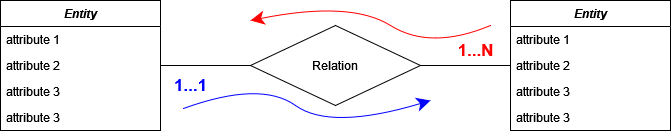
\includegraphics[width=0.6\textwidth]{legendaER.png}
	\caption{ER Diagram Organization}
	\label{fig:erleg}
\end{figure}
\bigskip
\begin{figure}[H]
	\centering
	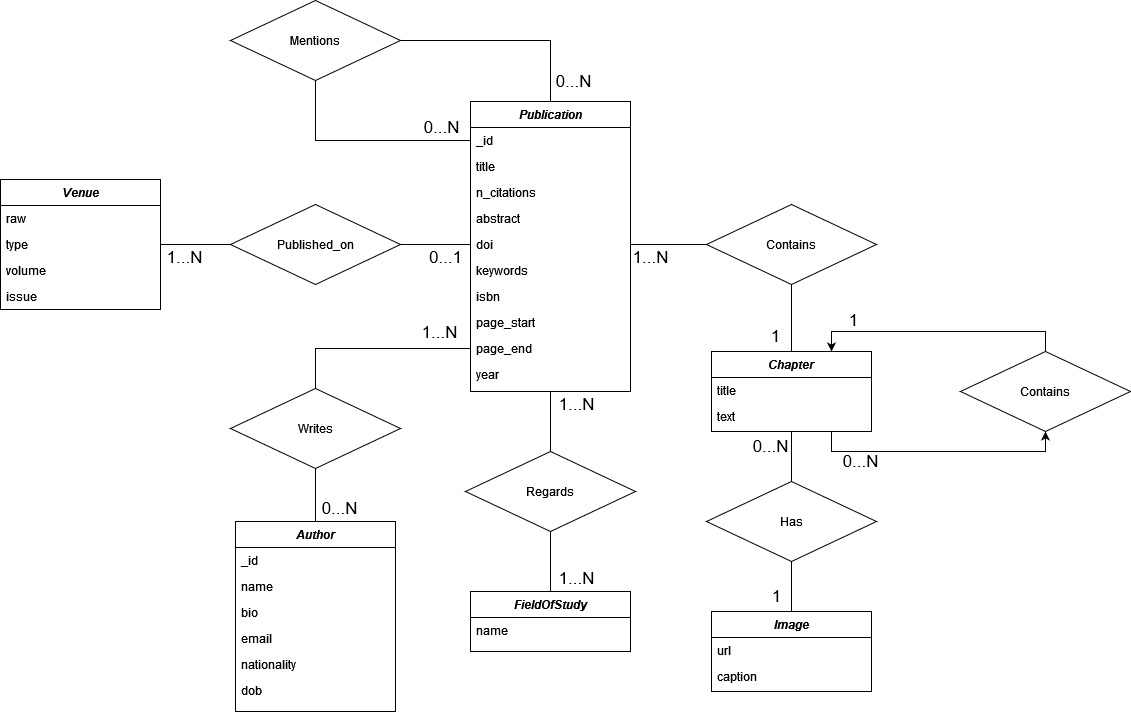
\includegraphics[width=1\textwidth]{ERDocDb.png}
	\caption{ER Diagram}
	\label{fig:er}
\end{figure}


\chapter{Sample Dataset}
\label{ch:sample_dataset}
\begin{lstlisting}[language=json,firstnumber=1]
{
	"_id": {
		"_id": "53e99f86b7602d9702859fdf"
	},
	"title": "Locality Sensitive Outlier Detection: A ranking driven approach",
	"authors": [
	{
		"name": "Ye Wang",
		"org": "Computer Science and Engineering Department, The Ohio State University, USA"
	},
	{
		"name": "Srinivasan Parthasarathy",
		"org": "Computer Science and Engineering Department, The Ohio State University, USA"
	},
	{
		"name": "Shirish Tatikonda",
		"org": "Computer Science and Engineering Department, The Ohio State University, USA"
	}
	],
	"n_citation": 60,
	"abstract": "Outlier detection is fundamental..."
	"doi": "10.1109/ICDE.2011.5767852",
	"keywords": [
		"database point",
		"ranking scheme",
		"geometric approach",
		...
	],
	"isbn": "978-1-4244-8958-9",
	"page_start": "410",
	"page_end": "421",
	"year": 2011,
	"fos": [
		"Locality-sensitive hashing",
		"Anomaly detection",
		"Data mining",
		...
	],
	"venue": {
		"raw": "ICDE",
		"type": 0,
		"volume": "",
		"issue": "",
		"publisher": null
	},
	"chapters": [{
		"title": "1. Introduction",
		"text": "Complicated domain one-to-one and..."
		"images": [
			{
				"caption": "Nena",
				"link": "https://image.tmdb.org..."
			},
			{
				"caption": "Banking On Bitcoin",
				"link": "https://image.tmdb.org..."
			},
			...
		]
	}],
	"references": [
		{
			"_id": "53e99fddb7602d97028b7e65"
		}
	]
}
\end{lstlisting}


\end{document}
